\chapter{Orthophotos 1977-2023}\label{app:orthophotos}

\begin{figure}[p]
    \centering
    \includegraphics[height=\textheight]{figures/appendix/orto_1977.jpg}
    \caption[][]{Historical-aerial orthophoto from 1977.}
\end{figure}

\begin{figure}[p]
    \centering
    \includegraphics[height=\textheight]{figures/appendix/orto_1991.jpg}
    \caption[]{Historical-aerial orthophoto from 1991.}
\end{figure}

\begin{figure}[p]
    \centering
    \includegraphics[height=\textheight]{figures/appendix/orto_2001.jpg}
    \caption[]{Historical-aerial orthophoto from 2001.}
\end{figure}

\begin{figure}[p]
    \centering
    \includegraphics[height=\textheight]{figures/appendix/orto_2009.jpg}
    \caption[]{Aerial orthophoto from 2009.}
\end{figure}

\begin{figure}[p]
    \centering
    \includegraphics[height=\textheight]{figures/appendix/orto_2015.jpg}
    \caption[]{UAV orthophoto from 2015.}
\end{figure}

\begin{figure}[p]
    \centering
    \includegraphics[height=\textheight]{figures/appendix/orto_2016.jpg}
    \caption[]{UAV orthophoto from 2016.}
\end{figure}

\begin{figure}[p]
    \centering
    \includegraphics[height=\textheight]{figures/appendix/orto_2017.jpg}
    \caption[]{UAV orthophoto from 2017.}
\end{figure}

\begin{figure}[p]
    \centering
    \includegraphics[height=\textheight]{figures/appendix/orto_2018.jpg}
    \caption[]{UAV orthophoto from 2018.}
\end{figure}

\begin{figure}[p]
    \centering
    \includegraphics[height=\textheight]{figures/appendix/orto_2019.jpg}
    \caption[]{UAV orthophoto from 2019.}
\end{figure}

\begin{figure}[p]
    \centering
    \includegraphics[height=\textheight]{figures/appendix/orto_2020.jpg}
    \caption[]{UAV orthophoto from 2020.}
\end{figure}

\begin{figure}[p]
    \centering
    \includegraphics[height=\textheight]{figures/appendix/orto_2021.jpg}
    \caption[]{UAV orthophoto from 2021.}
\end{figure}

\begin{figure}[p]
    \centering
    \includegraphics[height=\textheight]{figures/appendix/orto_2022.jpg}
    \caption[]{UAV orthophoto from 2022.}
\end{figure}

\begin{figure}[p]
    \centering
    \includegraphics[height=\textheight]{figures/appendix/orto_2023.jpg}
    \caption[]{UAV orthophoto from 2023.}
\end{figure}

% \chapter{DSMs}\label{app:dsm}

% \begin{figure}[p]
%     \centering
%     \includegraphics[width=\textwidth]{figures/chapter3/orto2015.jpg}
%     \caption[]{UAV-based orthophoto 2015}
% \end{figure}

% \begin{figure}
%     \centering
%     \includegraphics[width=\textwidth]{figures/chapter3/orto2016.jpg}
% \end{figure}

\chapter{Surface velocity fields 2015-2023}\label{app:sfv}

\begin{figure}[p]
    \centering
    \includegraphics[height=\textheight]{figures/chapter3/velocity_DIC_2015-2016.png}
    \caption[]{Glacier surface velocity field derived by DIC on DSM 2015-2016}
\end{figure}

\begin{figure}
    \centering
    \includegraphics[height=\textheight]{figures/chapter3/velocity_DIC_2016-2017.png}
    \caption[]{Glacier surface velocity field derived by DIC on DSM 2016-2017}
\end{figure}

\begin{figure}
    \centering
    \includegraphics[height=\textheight]{figures/chapter3/velocity_DIC_2017-2018.png}
    \caption[]{Glacier surface velocity field derived by DIC on DSM 2017-2018}
\end{figure}

\begin{figure}
    \centering
    \includegraphics[height=\textheight]{figures/chapter3/velocity_DIC_2018-2019.png}
    \caption[]{Glacier surface velocity field derived by DIC on DSM 2018-2019}
\end{figure}

\begin{figure}
    \centering
    \includegraphics[height=\textheight]{figures/chapter3/velocity_DIC_2019-2020.png}
    \caption[]{Glacier surface velocity field derived by DIC on DSM 2019-2020}
\end{figure}

\begin{figure}
    \centering
    \includegraphics[height=\textheight]{figures/chapter3/velocity_DIC_2020-2021.png}
    \caption[]{Glacier surface velocity field derived by DIC on DSM 2020-2021}
\end{figure}

\begin{figure}
    \centering
    \includegraphics[height=\textheight]{figures/chapter3/velocity_DIC_2021-2022.png}
    \caption[]{Glacier surface velocity field derived by DIC on DSM 2021-2022}
\end{figure}

\begin{figure}
    \centering
    \includegraphics[height=\textheight]{figures/chapter3/velocity_DIC_2022-2023.png}
    \caption[]{Glacier surface velocity field derived by DIC on DSM 2022-2023}
\end{figure}


\chapter{Cross-sections}\label{app:xsec}

\begin{figure}[p]
    \centering
    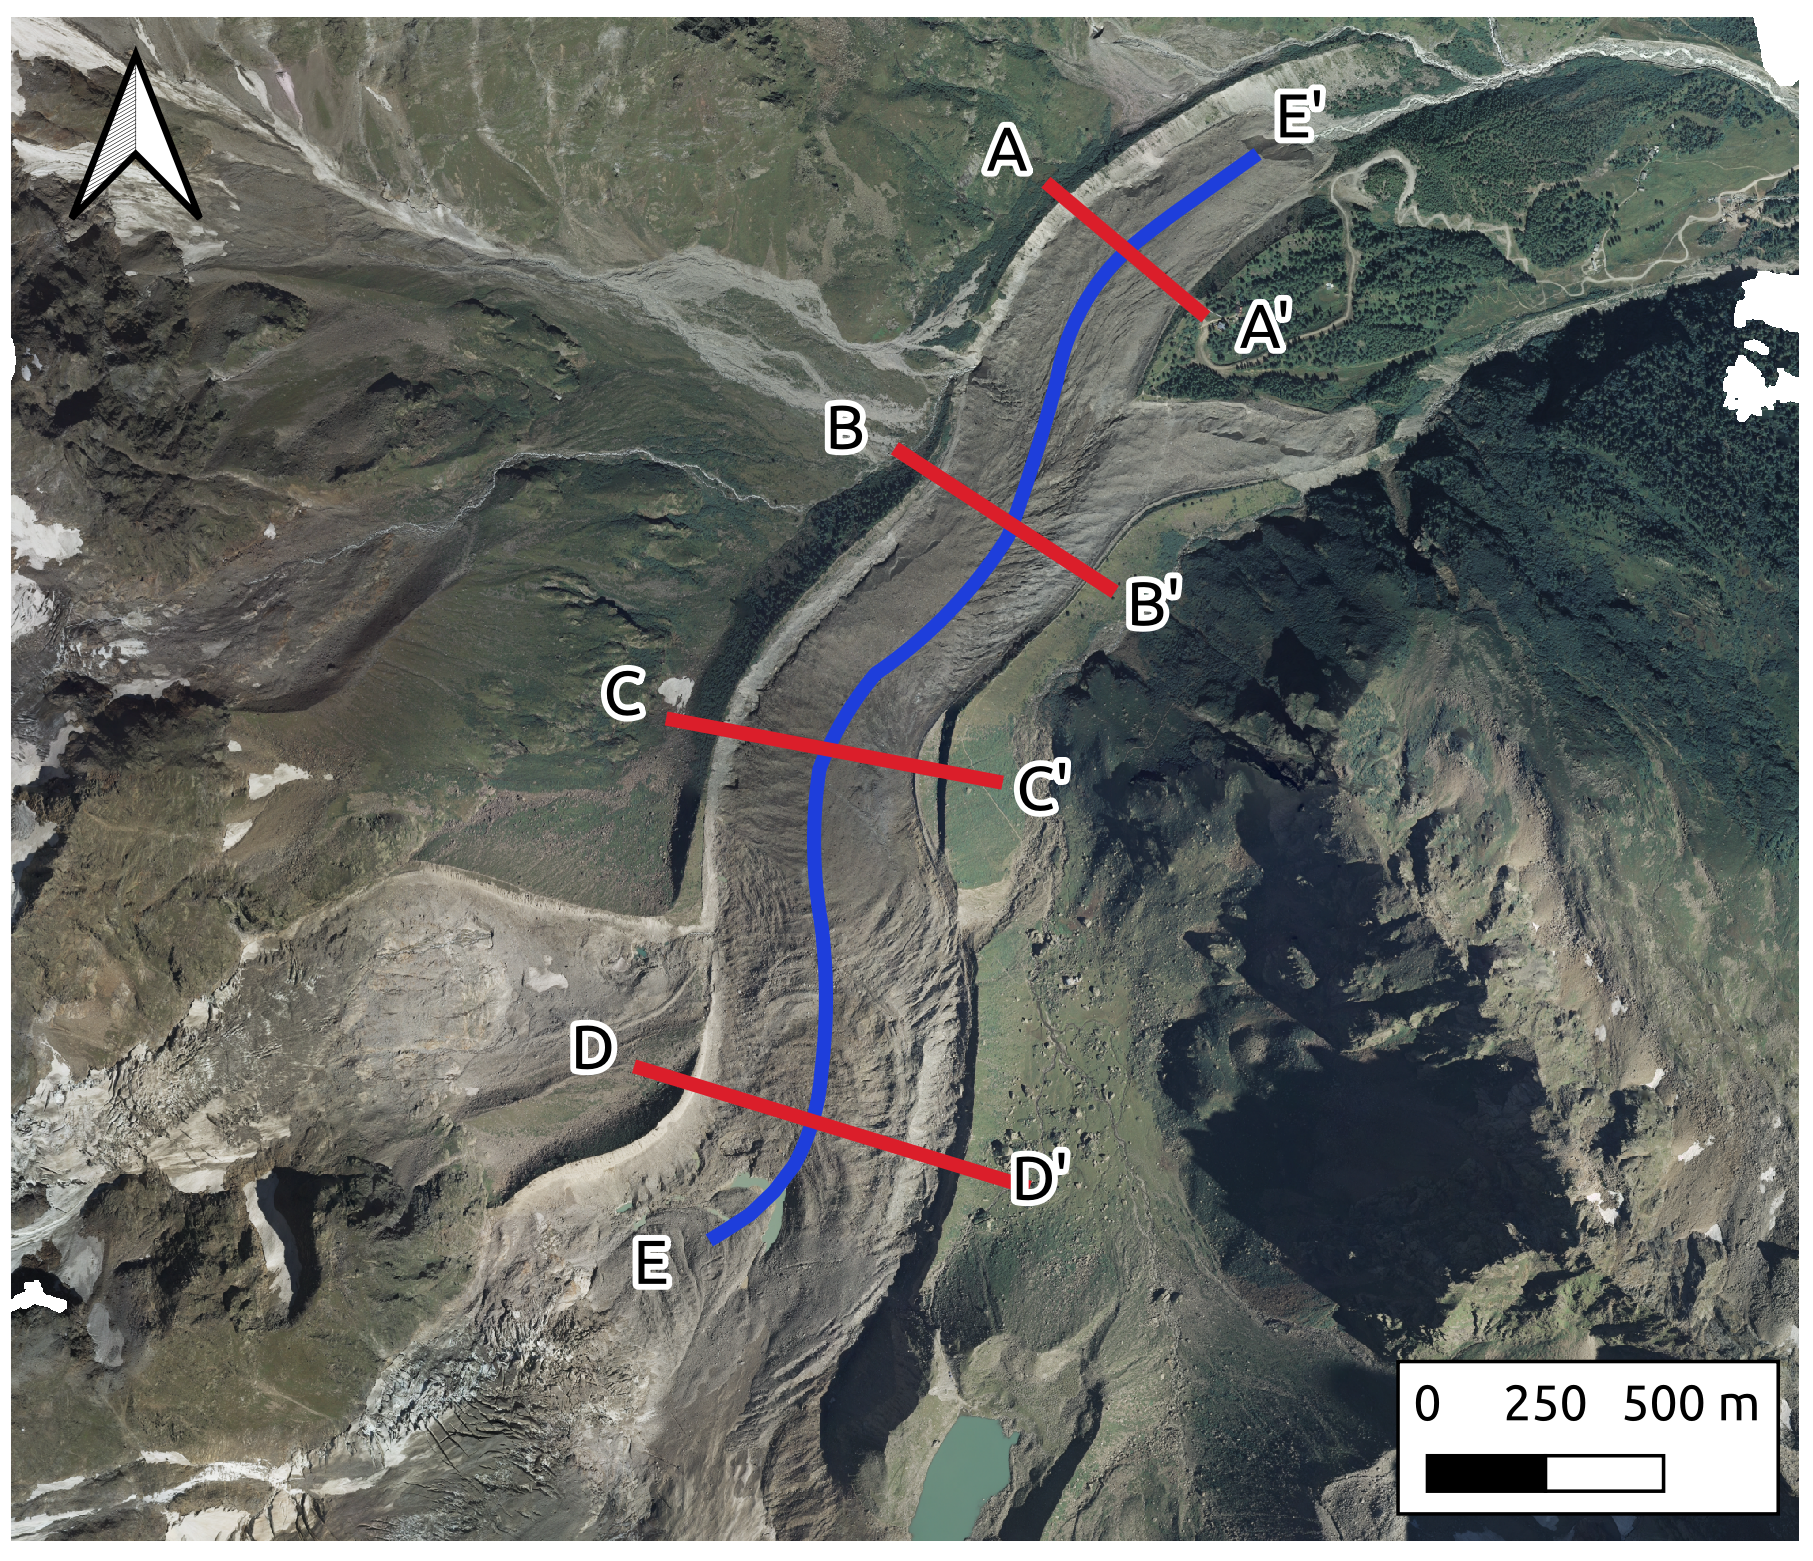
\includegraphics[width=\textwidth]{figures/chapter3/profiles_map.png}\\
    \caption[]{Location of the cross-sections}
\end{figure}

\begin{figure}[p]
    \centering
    \includegraphics[width=\textwidth]{figures/appendix/profile_A.jpg}\\
    \includegraphics[width=0.7\textwidth]{figures/chapter3/profiles_legend.png}
    \caption[]{Cross sections along the profile AA'}
\end{figure}

\begin{figure}[p]
    \centering
    \includegraphics[width=\textwidth]{figures/appendix/profile_B.jpg}\\
    \includegraphics[width=0.7\textwidth]{figures/chapter3/profiles_legend.png}
    \caption[]{Cross sections along the profile BB'}
\end{figure}

\begin{figure}[p]
    \centering
    \includegraphics[width=\textwidth]{figures/appendix/profile_C.jpg}\\
    \includegraphics[width=0.7\textwidth]{figures/chapter3/profiles_legend.png}
    \caption[]{Cross sections along the profile CC'}
\end{figure}

\begin{figure}[p]
    \centering
    \includegraphics[width=\textwidth]{figures/appendix/profile_D.jpg}\\
    \includegraphics[width=0.7\textwidth]{figures/chapter3/profiles_legend.png}
    \caption[]{Cross sections along the profile DD'}
\end{figure}

\begin{figure}[p]
    \centering
\includegraphics[height=\textheight]{figures/appendix/profile_flow_rot.png}
    \caption[]{Cross sections along the profile EE', extracted along the glacier flow direction.}
\end{figure}

\chapter{Camera residuals}\label{app:camera_res}

This appendix presents the residual images for the various cameras used in the photogrammetric blocks throughout the thesis. 
These residual images, as computed by Agisoft Metashape, represent the reprojection error of the tie points averaged within a regular grid in the image and averaged across all the images associated with each camera.

The reprojection errors are depicted as vectors, with colors indicating the magnitude of the error: green denotes lower error, while red indicates higher error.
The scale of these vectors is provided in each plot via a scalebar located below the figure, expressed in millimeters for cameras with fiducial marks (such as the analog cameras used in Chapter \ref{ch:2}) or pixels for digital cameras. 
Additionally, the RMS and the maximum reprojection errors are reported for each camera.

Some systematic errors are visible in some of the residual plots at the edges of the image, particularly with lower-quality cameras. 
However, the RMS values of the residuals are consistently significantly below the pixel level, with maximum residuals generally not exceeding \SI{2}{\pixel}.

\begin{figure}[hb]
  \centering
  \subcaptionbox{1977 - Wild RC10 - 15 UAG I 153.260 mm}{
    \includegraphics[trim={0 0 0 2mm},clip,height=6cm]{figures/appendix/camera_residuals_1977}
  } \qquad
  \subcaptionbox{1991}{
    \includegraphics[trim={0 0 0 2mm},clip,height=6cm]{figures/appendix/camera_residuals_1991}
  } \\ \vspace{2mm}
  \subcaptionbox{2001}{
    \includegraphics[trim={0 0 0 2mm},clip,height=6cm]{figures/appendix/camera_residuals_2001}
  } \qquad
  \subcaptionbox{2009}{
    \includegraphics[trim={0 0 0 2mm},clip,height=6cm]{figures/appendix/camera_residuals_2009}
  } \\ \vspace{2mm}
  \subcaptionbox{2019}{
    \includegraphics[trim={0 0 0 2mm},clip,height=6cm]{figures/appendix/camera_residuals_2019}
  } \\  
  \caption[]{Residual image for the cameras employed for reconstructing the glacier in 1977, 1991, 2001, 2009, and 2019 as described in Chapter \ref{ch:2}.}
  \label{fig:app:camera_residuals_histo}
\end{figure}

\begin{figure}[hb]
  \centering
  \subcaptionbox{2015 - Canon PowerShot S110}{
    \includegraphics[trim={0 0 0 2mm},clip,height=5.5cm]{figures/appendix/2015_S110.png}
  } \quad
  \subcaptionbox{2016 - Canon PowerShot S110}{
    \includegraphics[trim={0 0 0 2mm},clip,height=5.5cm]{figures/appendix/2016_S110.png}
  } \\ \vspace{2mm}
  \subcaptionbox{2017 - Canon PowerShot S110}{
    \includegraphics[trim={0 0 0 2mm},clip,height=5.5cm]{figures/appendix/2017_S110.png}
  } \quad
  \subcaptionbox{2017 - SenseFly S.O.D.A}{
    \includegraphics[trim={0 0 0 2mm},clip,height=5.5cm]{figures/appendix/2017_SODA.png}
  } \\ \vspace{2mm}
  \subcaptionbox{2017 - DJI Phantom 4 (DJI FC6310)}{
    \includegraphics[trim={0 0 0 2mm},clip,height=5.5cm]{figures/appendix/2017_ph4.png}
  } 
  \caption[]{Residual image for the cameras employed for the annual UAV reconstruction, described in Chapter \ref{ch:3}.}
  \label{fig:app:camera_residuals_uav1}
\end{figure}

\begin{figure}[ht]
  \centering
  \subcaptionbox{2018 - Hawkeye Firefly 8S}{
    \includegraphics[trim={0 0 0 2mm},clip,height=5.5cm]{figures/appendix/2018_firefly.png}
  } \quad
  \subcaptionbox{2019 - Hawkeye Firefly 8S}{
    \includegraphics[trim={0 0 0 2mm},clip,height=5.5cm]{figures/appendix/2019_firefly.png}
  } \\ \vspace{2mm} 
  \subcaptionbox{2020 - Hawkeye Firefly 8S}{
    \includegraphics[trim={0 0 0 2mm},clip,height=5.5cm]{figures/appendix/2020_firefly.png}
  } \quad
  \subcaptionbox{2021 - DJI ZenMuse X5S - 15 mm}{
    \includegraphics[trim={0 0 0 2mm},clip,height=5.5cm]{figures/appendix/2021_x5s.png}
  } \\ \vspace{2mm}
  \caption[]{Residual image for the cameras employed for the annual UAV reconstruction, described in Chapter \ref{ch:3}.}
  \label{fig:app:camera_residuals_uav2}
\end{figure}

\begin{figure}[ht]
  \centering
  \subcaptionbox{2022 - DJI Zenmuse P1 - 35 mm (glacier)}{
    \includegraphics[trim={0 0 0 2mm},clip,height=5.5cm]{figures/appendix/2022_p1_ghiacc.png}
  } \quad
  \subcaptionbox{2022 - DJI Zenmuse P1 - 35 mm (north-west lobe)}{
    \includegraphics[trim={0 0 0 2mm},clip,height=5.5cm]{figures/appendix/2022_p1_lingua.png}
  } \\ \vspace{2mm}
  \subcaptionbox{2022 - Phantom 4 RTK (DJI FC6310)}{
    \includegraphics[trim={0 0 0 2mm},clip,height=5.5cm]{figures/appendix/2022_ph4.png}
  } \quad
  \subcaptionbox{2023 - DJI Zenmuse P1 - 35 mm}{
    \includegraphics[trim={0 0 0 2mm},clip,height=5.5cm]{figures/appendix/2023_p1.png}
  } \\ \vspace{2mm}
  \caption[]{Residual image for the cameras employed for the annual UAV reconstruction, described in Chapter \ref{ch:3}.}
  \label{fig:app:camera_residuals_uav3}
\end{figure}

\begin{figure}[hb]
  \centering
  \subcaptionbox{Camera C1 - calibration}{
    \includegraphics[trim={0 0 0 2mm},clip,height=5.5cm]{figures/appendix/c1_calib.png}
  } \quad
  \subcaptionbox{Camera C2 - calibration}{
    \includegraphics[trim={0 0 0 2mm},clip,height=5.5cm]{figures/appendix/c2_calib.png}
  } \\ \vspace{2mm}
  \subcaptionbox{Camera C1 - 01/06/2022}{
    \includegraphics[trim={0 0 0 2mm},clip,height=5.5cm]{figures/appendix/c1_010622.png}
  } \quad
  \subcaptionbox{Camera C2 - 01/06/2022}{
    \includegraphics[trim={0 0 0 2mm},clip,height=5.5cm]{figures/appendix/c2_010622.png}
  } \\ \vspace{2mm}
  \caption[]{Residual images for the fixed stereo cameras used for daily reconstruction of the glacier terminus, as described in Chapter \ref{ch:2}. The top row displays the residual images during the calibration process, which was conducted by integrating the stereo images within a complete UAV block and using GCPs (see \secref{sec:4}. The bottom row provides an example of the residual images for a single epoch (01/06/2022). In this case, the camera's interior orientation was fixed to the pre-calibrated values, except for the principal distance (focal length), which was refined through self-calibration.}
  \label{fig:app:camera_residuals_stereocams}
\end{figure}

